\input umk_preamble

\input general_info.tex

\begin{document}

%\tableofcontents

\section{Цели и задачи освоения дисциплины}

\textbf{Целью} данного курса является знакомство студентов с основными принципами функционирования вычислительных систем, а также с проблематикой их проектирования. В рамках курса решаются следующие \textbf{задачи}.
\begin{itemize}
	\item Знакомство с основными этапами исторического развития вычислительной техники.
	\item Изложение современного подхода к изучению компьютерных системы.
	\item Выделение среди общего многообразия компьютеров основных типов и различий в принципах их устройства.
	\item Определение роли каждого из основных компонентов вычислительной системы в её организации, а также проблем, связанных с их проектированием.
	\item Изучение основных примитивов цифровой логики и способов их объединения.
	\item Изложение принципа микропрограммного управления на примере конкретной микроархитектуры.
	\item Определение способа представления чисел в памяти машин.
	\item Описание ключевой роли уровня набора инструкций, как интерфейса между аппаратным и программным обеспечением.
	\item Знакомство с базовыми инструкциями из набора x86 с помощью программирования на языке ассемблера.
\end{itemize}

\section{Место дисциплины в структуре ООП ВПО}

% использовать \ssect[Абв] или \ssect для нумерации подразделов
% с факультативным заголовком

	\ssect Учебная дисциплина \thecourse{}
(\theyearofstudy~курс, \theterm~семестр) относится к \ulinepad{
% математическому и естественнонаучному%
% /
профессиональному%
% обычно видно по учебному плану:
% м. и ес. там обозначен Б2, п. -- Б3
% учебные планы ЮФУ: http://sfedu.ru/www/view_plans.startup
} циклу.

	\ssect % пререквизиты, например:
Для изучения курса \thecourse{} (\theyearofstudy~курс, \theterm~семестр)
студенту достаточно владеть навыками программирования на одном из императивных языков, например, Pascal или C. К особо важным темам базовых курсов по программированию, понимание которых используется в данном курсе, следует отнести следующие:
\begin{itemize}
	\item указатели и прямая работа с памятью,
	\item организация типа данных <<массив>>,
	\item устройство структуры данных <<линейный односвязный список>>.
\end{itemize}

	\ssect
В дальнейшем материал данного курса может использоваться в ряде курсов,
изучаемых на 3--4 курсах, в том числе: компьютерные сети, операционные системы, теория автоматов и формальных языков, параллельное и многопоточное
программирование.

\section{Требования к результатам освоения содержания дисциплины}

	\ssect
Процесс изучения дисциплины направлен на формирование элементов следующих компетенций в соответствии с ФГОС ВПО (ОС ЮФУ) и ООП ВПО по данному направлению подготовки:
% общий перечень компетенций по направлению подготовки обычно
% можно найти в госстандарте или в ООП вуза. ФГОСы размещены на одном из
% специализированных сайтов Минобра. Сейчас это:
% http://fgosvo.ru/fgosvpo/7/6/1/28
% ООП направлений ЮФУ должны быть на офсайте
% на данный момент (середина 2014) это:
% http://sfedu.ru/www/edu.NaprPodg_show?v_snp_date_in=01.01.2009
% существующий на данный момент перечень для ПМИ и ФИИТ вынесен в файл:
% https://docs.google.com/document/d/12WMvvjyVEkF9S5gQVCI26zMnVXGQJcVEv18Qjz_x9yk/edit?usp=sharing
\begin{enumerate}
\rusitems % нумерация кириллическими буквами
	\item общекультурных (ОК):
	\begin{itemize}
		\item уважительно и бережно относиться к историческому наследию и культурным традициям, толерантно воспринимать социальные и культурные различия (ОК-2);
		\item понимать движущие силы и закономерности исторического процесса; роль насилия и ненасилия в истории, место человека в историческом процессе, политической организации общества (ОК-3);
		\item способность критически переосмысливать накопленный опыт, изменять при необходимости вид и характер своей профессиональной деятельности (ОК-8);
		\item способность работать с информацией в глобальных компьютерных сетях (ОК-13);
	\end{itemize}

	\item профессиональных (ПК):
	\begin{itemize}
		\item способность применять на практике международные и профессиональные стандарты информационных технологий, современные парадигмы и методологии, инструментальные и вычислительные средства (ПК-7);
		\item способность профессионально владеть базовыми математическими знаниями и информационными технологиями, эффективно применять их для решения научно-технических задач и прикладных задач, связанных с развитием и использованием информационных технологий (ПК-8);
		\item способность решать задачи производственной и технологической деятельности на высоком профессиональном уровне, включая: разработку алгоритмических и программных решений в области системного и прикладного программирования; разработку математических, информационных и имитационных моделей по тематике выполняемых опытно-конструкторских работ и проектов; создание информационных ресурсов глобальных сетей, образовательного контента, прикладных баз данных; разработку тестов и средств тестирования систем и средств на соответствие стандартам и исходным требованиям; разработку эргономичных человеко-машинных интерфейсов в соответствии с профилями подготовки (ПК-28).
	\end{itemize}
\end{enumerate}

В результате освоения дисциплины обучающийся должен

\noindent\textbf{знать:}
	\begin{itemize}[topsep=1mm]
		\item основные этапы развития вычислительной техники,
		\item примеры применения компьютеров в современном обществе,
		\item наиболее широкоупотребительные способы классификации компьютеров,
		\item составляющие части вычислительной системы и проблематику их разработки и взаимодействия,
		\item уровни архитектуры современной вычислительной машины, их назначение и взаимодействие,
		\item основные цифровые логические схемы и шины, используемые в компьютерах,
		\item проблематику микропрограммного управления центральным процессором,
		\item задачи, решаемые уровнем набора инструкций,
		\item способы представления целых знаковых чисел в компьютере,
		\item способы представления рациональных чисел в компьютере: числа с фиксированной точкой, числа с плавающей точкой, стандарт IEEE~754,
		\item ядро набора инструкций x86;
	\end{itemize}

\clearpage
\noindent\textbf{уметь:}
	\begin{itemize}[topsep=1mm]
		\item различать вычислительные машины, относящиеся к разным поколениям,
		\item определять тип вычислительной архитектуры в каждой из основных классификаций: фоннеймановская/гарвардская, CISC/RISC, SISD/SIMD/MISD/MIMD,
		\item определять представление целых беззнаковых чисел в машинах с различной организацией ОЗУ: разным размером байт и разным порядком байт в слове,
		\item использовать простейшие помехоустойчивые коды: проверки чётности, (7,4)"/Хэм\-мин\-га,
		\item прогнозировать поведение простейших цифровых логических схем,
		\item составлять фрагменты микропрограммы для простейших микроархитектур,
		\item определять представление целых знаковых чисел и чисел с плавающей точкой по стандарту IEEE~754 в памяти компьютера,
		\item составлять простейшие программы на языке ассемблера для процессора семейства x86;
	\end{itemize}

\noindent\textbf{владеть:}
	\begin{itemize}[topsep=1mm]
		\item терминологией из области архитектуры компьютера,
		\item средствами ассемблирования программ.
	\end{itemize}

\section{Содержание и структура дисциплины}

%	\ssect[Содержание модулей дисциплины]

% общая информация о модулях должна быть представлена в данном файле:
\input my_units.tex

% для изложения содержания каждого модуля используется команда myunit,
%   она создаёт бокс с рамкой, это отличается от табличного формата,
%   данного в образце УМК/РПД, однако их формат:
%   1) неразумно использует пространство страницы (пустые колонки)
%   2) сложно или невозможно воспроизвести в LaTeX,
%		см. http://tex.stackexchange.com/q/192728/7460

%	имена модулей должны быть заданы в файле my_units.tex
%		здесь указывается только содержание и формы контроля

%	Главный корпус требует от 2 до 4 модулей (включительно)

% Вступительная фраза и две таблицы с расчасовками:
%\printhours

\begin{landscape}
\pagestyle{empty}

\begin{table}[h]
\caption{Структура дисциплины}
\centering
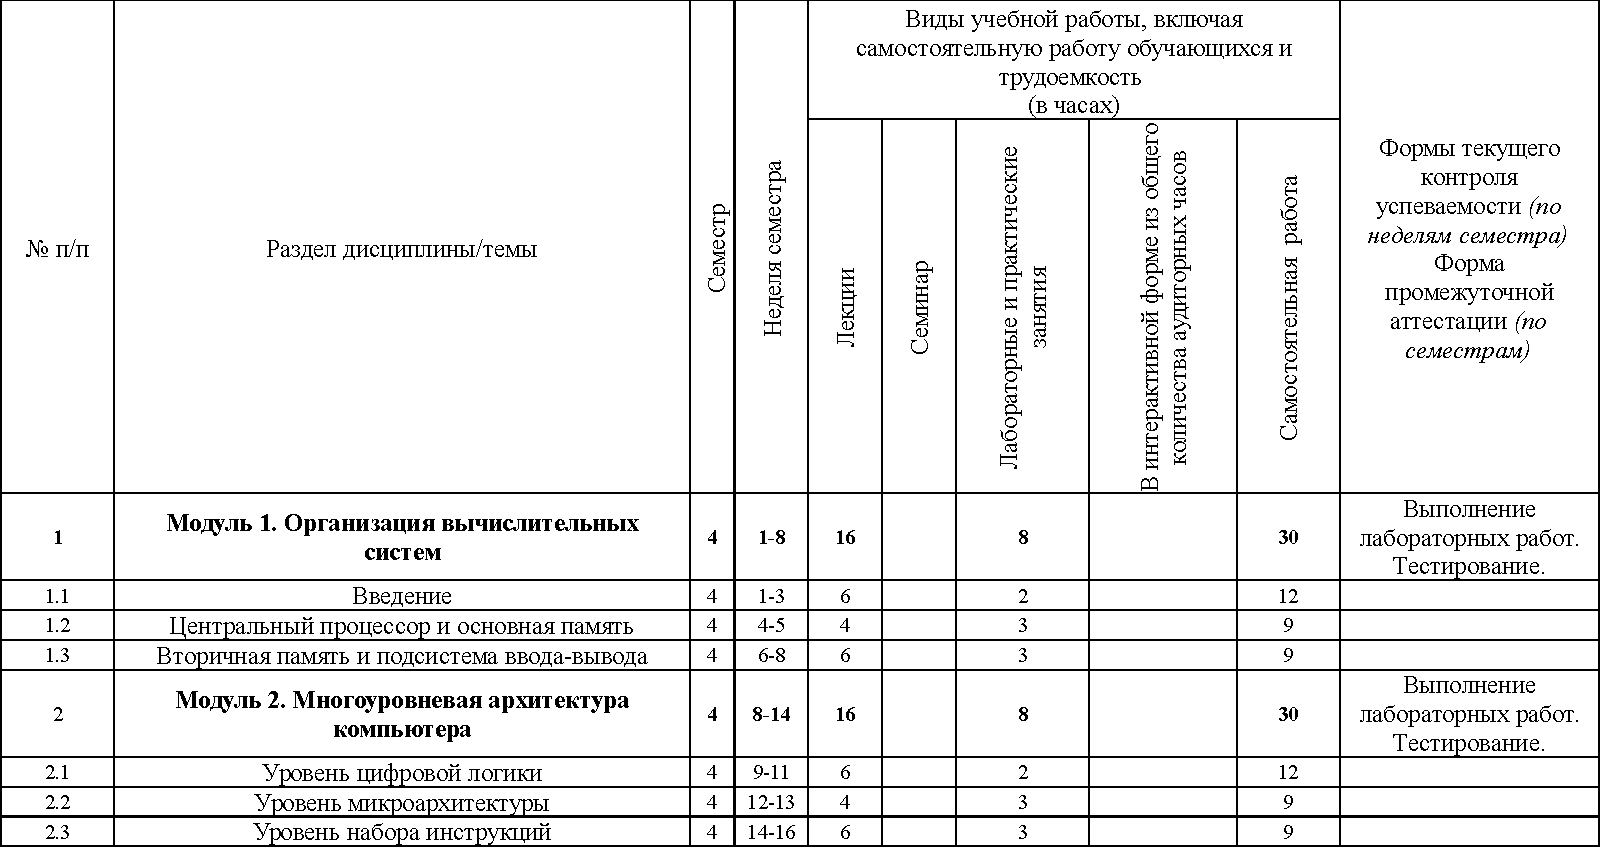
\includegraphics[width=\linewidth]{t1.pdf}
\end{table}

%\ssect[]

\begin{table}[h]
\caption{План внеаудиторной самостоятельной работы обучающихся по дисциплине}
\centering
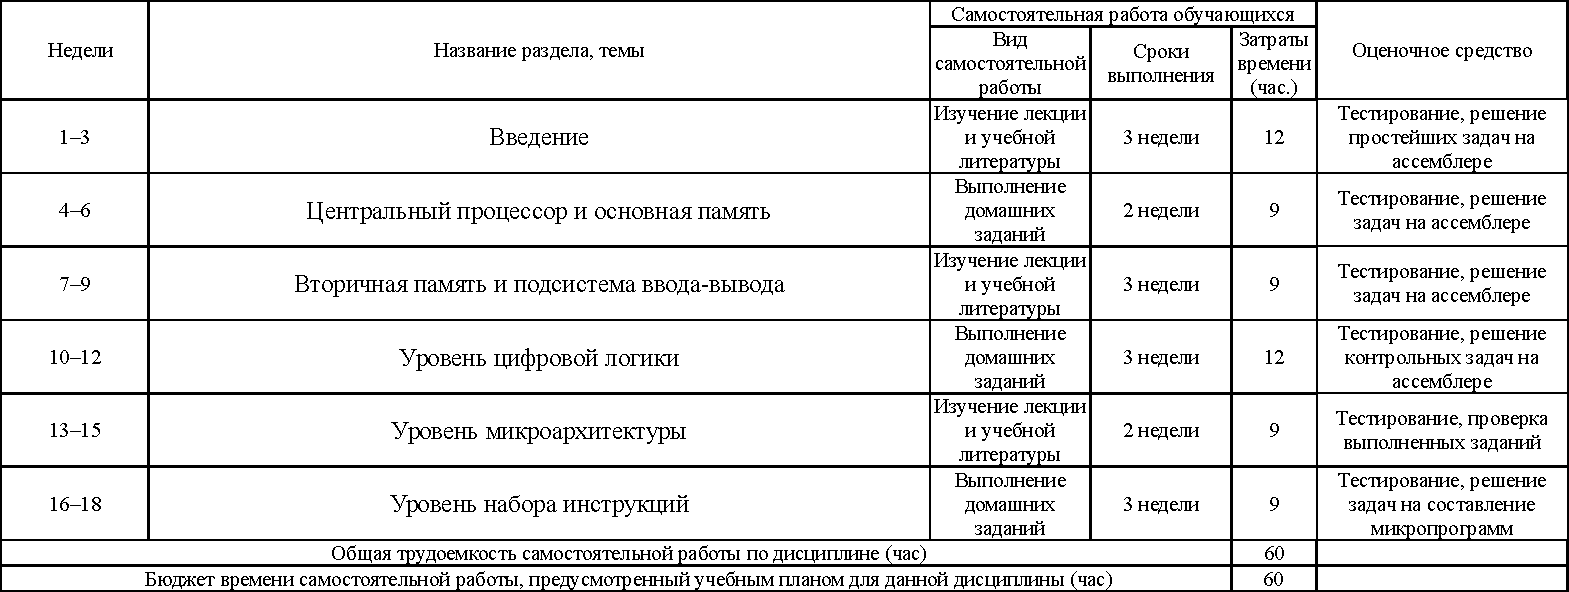
\includegraphics[width=\linewidth]{t2.pdf}
\end{table}
\end{landscape}


%\mylab{Имя лабы}{часы}
%~ \printlabs{%
	%~ \mylab{Простейшие программы, арифметика и циклы LOOP}{2}%
	%~ \mylab{Массивы. Условные и безусловные переходы}{2}%
	%~ \mylab{Интерфейс системных вызовов. Простейшие подпрограммы}{2}%
	%~ \mylab{Подпрограммы (продолжение)}{2}%
	%~ \mylab{Цепочечные инструкции}{2}%
	%~ \mylab{Контрольная лабораторная работа}{2}%
	%~ %
	%~ \incMyunit
	%~ %
	%~ \mylab{Работа с файлами}{2}%
	%~ \mylab{Микропрограммирование}{2}%
%~ }

\section{Образовательные технологии}

Учебный курс состоит из двух учебных модулей. По окончании каждого модуля проводятся контрольные работы в виде электронных тестов для проверки усвоения теоретического материала и в виде задач для решения на компьютере по аналогии с задачами, выданными в рамках лабораторных работ. Лабораторные работы описаны в пособии [1] п.~\ref{author-res}.

При проведении лекций и практических занятий используются следующие образовательные технологии:
\begin{itemize}
	\item мультимедийные лекции;
	\item электронные формы контроля;
	\item самотестирование студентов.
\end{itemize}

Учебный процесс базируется на концепции компетентностного обучения, ориентированного на формирование конкретного перечня профессиональных компетенций, актуализацию получаемых теоретических знаний. Развертывание компетентностной модели обучения предполагает широкое применение инновационных способов организации учебного процесса, в том числе технологий управляемого самостоятельного обучения в том числе балльно-рейтинговой системы, а также внедрение системы онлайн-поддержки внеаудиторной работы студентов.

\section{Оценочные средства для текущего контроля успеваемости и промежуточной аттестации}

\emph{Полный комплект контрольно-оценочных материалов (Фонд оценочных средств) оформлен в виде приложения к рабочей программе дисциплины.}

\section{Учебно-методическое обеспечение дисциплины}

	\ssect[Основная литература]\label{main-lit}

\begin{enumerate}
	\item Tanenbaum A., Ostin T. Structured Computer Organization / Prentice Hall; 6th edition (August 4, 2012). 800 p.\\
	Перевод: Таненбаум Э., Остин Т. Архитектура компьютера / 6-е изд.(+CD) — СПб.: Питер, 2013. — 816 с.
\end{enumerate}

	\ssect[Дополнительная литература]
\begin{enumerate}
	\item Stallings W. Computer Organization and Architecture /  Prentice Hall; 9th edition (March 11, 2012). 792 p.\\
	Перевод: Столлингс У. Структурная организация и архитектура компьютерных систем / М: Вильямс, 2002. 896 с.
\end{enumerate}

	\ssect[Список авторских методических разработок]
	\label{author-res}
\begin{enumerate}
	\item А.\,М.~Пеленицын, Н.\,Н.~Ячменёва. Методические указания к практикуму по курсу «Архитектура компьютера» [Электронный ресурс]\\
	\url{http://open-edu.sfedu.ru/node/2622}
\end{enumerate}

	\ssect[Интернет-ресурсы]\label{online-res}
\begin{enumerate}
	\item Сопроводительные материалы к учебнику [1] п.~\ref{main-lit}:
	\begin{otherlanguage}{english}
	Structured Computer Organization, 6/E
	\end{otherlanguage}
	[Электронный ресурс]\\
	\url{http://www.pearsonhighered.com/educator/product/Structured-Computer-Organization-6E/9780132916523.page}

	\item Википедия: Свободная энциклопедия, английский раздел [Электронный ресурс]\\
	\url{http://en.wikipedia.org/wiki/Main_Page}
\end{enumerate}

\section{Материально-техническое обеспечение дисциплины}

	\ssect[Учебно-лабораторное оборудование]
Лекции проводятся в мультимедийном классе с презентационным оборудованием (проектором и экраном либо интерактивной доской). Лабораторные занятия проводятся в дисплейных классах с персональными компьютерами по числу, не уступающему числу студентов.

	\ssect[Программные средства]

Компьютеры в дисплейных классах должны быть снабжены операционной системой GNU/Linux, желательно в виде дружественного к пользователю дистрибутива (например, Ubuntu Linux).

На компьютерах в дисплейном классе должны быть распакованы в каталог \texttt{/bin} или \texttt{\textasciitilde/bin} три утилиты ассемблирования (as88/t88/s88) из сопроводительных материалов к учебнику Таненбаума (см. [1] в п.~\ref{online-res}). Для выполнения лабораторной работы по микропрограммированию необходимо наличие каталога Mic1MMV (с содержимым) оттуда же. Для его работы требуется виртуальная машина Java версии не ниже 1.4.

Для редактирования кода рекомендуется иметь установленным специализированный редактор с подсветкой синтаксиса языка ассемблера, например Geany или jEdit (оба находятся в частности в репозиториях Ubuntu Linux).

В отдельных случаях возможна работа на компьютерах под управлением операционной системы семейства Windows, однако здесь требуется дополнительная настройка утилит ассемблирования, описанная в методических указаниях~[1] п.~\ref{author-res}.


	\ssect[Технические и электронные средства]

Учёт активности студентов на курсе и основные материалы размещены в системе Moodle, развёрнутой в сети университета по адресу \url{http://edu.mmcs.sfedu.ru}. В дисплейных классах требуется доступ к этому ресурсу посредством браузера актуальной версии. Для проведения контрольных работ необходимо одновременно с доступом к указанному ресурсу ограничить доступ к другим интернет- и интранет-ресурсам, что на данный момент реализовано в лаборатории ММПТ и лаборатории кафедр алгебры и дискретной математики и информатики и вычислительного эксперимента факультета.

\clearpage
\section{Учебная карта дисциплины}

\input ukd_body.tex

\end{document}
